\documentclass[11pt]{article}

% Change "review" to "final" to generate the final (sometimes called camera-ready) version.
% Change to "preprint" to generate a non-anonymous version with page numbers.
\usepackage{acl}
\usepackage{float}
% Standard package includes
\usepackage{latexsym}
%Including images in your LaTeX document requires adding
%additional package(s)
\usepackage{graphicx}


% For proper rendering and hyphenation of words containing Latin characters (including in bib files)
% For Vietnamese characters
% \usepackage[T5]{fontenc}
% See https://www.latex-project.org/help/documentation/encguide.pdf for other character sets



% Arabic language support
\usepackage{fontspec}
\usepackage{polyglossia}
\setmainlanguage{english}
\setotherlanguage{arabic}
\newfontfamily\arabicfont[Script=Arabic]{Amiri}



% This is not strictly necessary, and may be commented out,
% but it will improve the layout of the manuscript,
% and will typically save some space.
\usepackage{microtype}

% This is also not strictly necessary, and may be commented out.
% However, it will improve the aesthetics of text in
% the typewriter font.
\usepackage{inconsolata}


\setmainfont{TeXGyreTermesX}

% If the title and author information does not fit in the area allocated, uncomment the following
%
%\setlength\titlebox{<dim>}
%
% and set <dim> to something 5cm or larger.

\title{BurhanAI at IslamicEval 2025 Shared Task: Combating Hallucinations in LLMs for Islamic Content; Evaluation,
Correction, and Retrieval-Based Solution}

% Author information can be set in various styles:
% For several authors from the same institution:
% \author{Author 1 \and ... \and Author n \\
%         Address line \\ ... \\ Address line}
% if the names do not fit well on one line use
%         Author 1 \\ {\bf Author 2} \\ ... \\ {\bf Author n} \\
% For authors from different institutions:
% \author{Author 1 \\ Address line \\  ... \\ Address line
%         \And  ... \And
%         Author n \\ Address line \\ ... \\ Address line}
% To start a separate ``row'' of authors use \AND, as in
% \author{Author 1 \\ Address line \\  ... \\ Address line
%         \AND
%         Author 2 \\ Address line \\ ... \\ Address line \And
%         Author 3 \\ Address line \\ ... \\ Address line}

\author{ 
        Arij Al Adel           \\  \texttt{arij.aladel@gmail.com}     \\\And   
        Abu Bakr Soliman       \\  \texttt{abubakr@rankxy.com}        \\\And
        Mohamed Sakher Sawan    \\ \texttt{me@sakher.co.uk}   \\\AND 
        Rahaf Al-Najjar         \\ \texttt{rahaf.m.alnajjar@gmail.com} \\\And
        Sameh Amin              \\ \texttt{Sameh.m.amin@gmail.com} \\     
} 
%\author{
%  \textbf{First Author\textsuperscript{1}},
%  \textbf{Second Author\textsuperscript{1,2}},
%  \textbf{Third T. Author\textsuperscript{1}},
%  \textbf{Fourth Author\textsuperscript{1}},
%\\
%  \textbf{Fifth Author\textsuperscript{1,2}},
%  \textbf{Sixth Author\textsuperscript{1}},
%  \textbf{Seventh Author\textsuperscript{1}},
%  \textbf{Eighth Author \textsuperscript{1,2,3,4}},
%\\
%  \textbf{Ninth Author\textsuperscript{1}},
%  \textbf{Tenth Author\textsuperscript{1}},
%  \textbf{Eleventh E. Author\textsuperscript{1,2,3,4,5}},
%  \textbf{Twelfth Author\textsuperscript{1}},
%\\
%  \textbf{Thirteenth Author\textsuperscript{3}},
%  \textbf{Fourteenth F. Author\textsuperscript{2,4}},
%  \textbf{Fifteenth Author\textsuperscript{1}},
%  \textbf{Sixteenth Author\textsuperscript{1}},
%\\
%  \textbf{Seventeenth S. Author\textsuperscript{4,5}},
%  \textbf{Eighteenth Author\textsuperscript{3,4}},
%  \textbf{Nineteenth N. Author\textsuperscript{2,5}},
%  \textbf{Twentieth Author\textsuperscript{1}}
%\\
%\\
%  \textsuperscript{1}Affiliation 1,
%  \textsuperscript{2}Affiliation 2,
%  \textsuperscript{3}Affiliation 3,
%  \textsuperscript{4}Affiliation 4,
%  \textsuperscript{5}Affiliation 5
%\\
%  \small{
%    \textbf{Correspondence:} \href{mailto:email@domain}{email@domain}
%  }
%}

\begin{document}
\maketitle


\begin{abstract}
In this paper, we describe our submission to the IslamicEval 2025 shared task, covering hallucination detection/correction and closed-world retrieval in Quranic and Hadith. We fine-tuned an LLM for detecting Quran and Hadith text spans, utilizing synthetic augmentation, diacritic variation, and morphological normalization to improve detection robustness (F1 = 87.10\%) and used another reasoning model with tools (F1 = 90.06\%). For validation, the accuracy is 88.60\%, and for correction the accuracy is 66.56\% where we employed a layered hierarchical index and search algorithm combining exact, normalized, fuzzy, and semantic matching with prompt-driven repair—to ensure canonical alignment and diacritic fidelity. For the correction stage, we also utilized a reasoning model with access to tools with an accuracy of 61.04\%. Regarding the ranked answer-bearing text retrieval task, we implemented a Retrieval-Augmented Generation (RAG) system restricted to the corpora provided by the shared task, with structured output, vector-store grounding, and prompts tuned for “answer-enclosing” citations that achieve MAP@10 of 0.6199 on the development set and 0.2807 on the test set. 
The results highlight the value of normalization, corpus-restricted search, and reasoning models with tools in mitigating hallucinations and improving retrieval precision in low-resource religious settings and that much smaller fine-tuned models can compete with frontier models (e.g. GPT-5 high) for specialized tasks such as span detection.

\end{abstract}

\section{Introduction}

Despite SOTA of large language models (LLMs) in a wide range of natural language processing (NLP) tasks, they frequently hallucinate \citet{Li2024BanishingLH, Hikal2025MSAAS, Orgad2024LLMsKM}.

Employing Large Language Models (LLMs) to process religious texts \citet{Ganadi2025GenerativeAF, Mohammed2025AftinaES} raises different ethical concerns, which makes it a topic of special interest within the Ethics of Natural Language Processing (NLP) \citet{Hutchinson2024ModelingTS}. In religious contexts, hallucinations can manifest as misquoted verses, fabricated Hadiths, or distorted interpretations, which pose significant ethical, theological, and social risks. Such errors may undermine public trust in AI systems and contribute to the spread of misinformation, particularly when dealing with sacred texts that have fixed, canonical forms.

Our main contributions to the IslamicEval-2025 \citet{mubarak2025islamiceval} shared task are threefold. First, we introduced a data pipeline to generate a synthetic dataset, enabling fine-tuning of a relatively small LLM (gpt-4.1-mini) for detecting spans of religious quotations—both claimed and correct. We benchmarked this approach against large reasoning models with access to a code interpreter, showing that the fine-tuned small model is cheaper and faster while maintaining strong performance. Second, we designed a layered hierarchical index and search algorithm, coupled with a low-cost LLM judge (gpt-4.1-mini), which outperformed a frontier reasoning model (GPT-5 with code interpreter) that is significantly slower and more expensive. Third, we developed a Retrieval-Augmented Generation (RAG) pipeline specialized for Quranic and Hadith question answering, tailored to the unique linguistic and semantic challenges of Islamic texts. We have released our GitHub repository publicly to facilitate transparency and reproducibility of our work \footnote{\url{https://github.com/sakher/IslamicEval-BurhanAI-Public}}. 



\section{Background}
We participated in Subtask 1A, which takes a model response as input and detects spans labeled Ayah or Hadith. In addition, we participated in Subtask 1B, which validates the spans identified in Subtask 1A labeling it as correct or incorrect, while Subtask 1C corrects any spans marked as incorrect by providing their correct form or flagging them as incorrect. Finally, Subtask 2 focuses on retrieving the top 20 answer-bearing citations from the Quran and Sahih Al-Bukhari given an Arabic question.


Many previous works have addressed hallucination in large language models using different approaches. 
One line of research applies Retrieval-Augmented Generation (RAG) \citet{Bechard2024ReducingHI,Alan2024ARQ, Khalila2025InvestigatingRG}. Other studies focus on instruction tuning and prompt engineering techniques \citet{Barkley2024InvestigatingTR, Hikal2025MSAAS}. 
Further research highlights verification and fact-checking strategies \citet{Sibaee2024ASOSAA}. 
Additionally, some works emphasize fine-tuning with human feedback \citet{Cheng2025ThinkMH,Lin2025Harnessing}. 
Together, these methods enable LLMs to function as more effective tools for factual verification and reliable information use.

\section{System Overview }
\subsection{Subtask 1A – Span Detection: }
We used two approaches; we fine‑tuned gpt‑4.1‑mini to output religious text spans. For fine-tuning we constructed a balanced training corpus (460 training examples and 83 validation examples) through multi-stage synthesis combining competition development data (70\%) with synthetic examples (30\%) generated using gpt-4.1 \footnote{ data generation pipeline \url{https://github.com/sakher/IslamicEval-BurhanAI-Public/blob/main/abubakr/taskA/01-index-religion-dataset-for-search.py}}. 

Separately, we leveraged a reasoning model with access to a code interpreter, testing both frontier and smaller OpenAI models (see detailed results in Table ~\ref{tab:1A}). The model was instructed to detect spans resembling Quran or Hadith. Since LLMs struggle with precise character counting \citet{fu2024large}, we enabled the code interpreter tool: whenever the model needed to compute exact offsets, it could generate Python code, which was then executed in a secure sandbox, and the resulting values were fed back into the model. This ensured reliable start and end indices for each span. Outputs were further constrained using the OpenAI API’s structured output feature with a JSON schema requiring a list of citations labeled as Ayah or Hadith with character offsets. We then applied heuristic post-processing: checking context within ±64 characters for lexical cues to refine labels, trimming extraneous punctuation or quotations, and merging or disentangling nested spans\footnote{ Prompts details \url{https://github.com/sakher/IslamicEval-BurhanAI-Public/blob/main/task_a_prompt_engineering/pipeline_task_a.py}}. 

\subsection{Subtask 1B – Validation and Subtask 1C – Correction: } \label{sec: val and corr}
Our system uses a layered design that combines seven forms of indexing with a six-stage search process. On the indexing side, every Quran verse and Hadith is indexed in multiple ways so the system can quickly switch between exact and approximate lookups. We keep exact MD5 hashes of the raw text, normalized versions without diacritics or punctuation, and character n-grams (3-grams by default) for fuzzy matches. Texts are also grouped into buckets by length to speed up candidate filtering, and we maintain a list for edit-distance checks. When available, we add a Whoosh full-text index for keyword search and a vector index built from Cohere embeddings stored in Qdrant for semantic similarity.

Searching happens in a strict sequence, with early stopping once a confident match is found. It starts with exact and normalized lookups, then falls back to n-gram fuzzy search. If needed, it escalates to semantic retrieval with embeddings and re-ranking. Next, it applies string-level fuzzy scorers such as Levenshtein distance and partial substring matching, followed by token-overlap checks to catch paraphrases. As a last resort, it computes Jaccard similarity on character trigrams. This stepwise design ensures clean matches are resolved instantly, while noisy, partial, or corrupted quotations are still recovered through progressively more flexible methods.

For the 1C correction subtask, we also tested a separate approach using a reasoning model - GPT-5 with high reasoning effort with access to tools. We give the model access to a code interpreter tool and to the corpora as text files. The model could perform multiple text-matching searches in the files to find the right match, then decide whether the matches were found  to return them in JSON format.

%\subsubsection{Subtask 1C – Correction: }
\subsection{Subtask 2 }
For Subtask 2, we built a Retrieval-Augmented Generation (RAG) system that retrieves passages from the Quran and Sahih Al-Bukhari. The corpora were split into 1,500-token chunks with 400-token overlap and stored as a vector dataset, allowing the reasoning model (GPT-5 with high reasoning) to run multiple searches per query when needed. The model could reformulate queries across iterations and returned ranked citations based on how directly and completely they answered the question. A deterministic post-processing pipeline then mapped Quran ayat to QPC \citet{malhas2020ayatec} passage IDs, validated hadith IDs against the official JSONL, removed duplicate citations.

\section{Experimental Setup}
    All results were against test dataset and as seen on CodaBench. Our systems included a fine-tuned span detector (gpt-4.1-mini, 3 epochs, batch size 1, LR multiplier 2.0, temp 0). Implementation utilizes \textbf{Whoosh} for inverted indexing, \textbf{FuzzyWuzzy} for edit distance computation, \textbf{Qdrant} for vector storage, \textbf{Cohere embed-v4.0} for embeddings, \textbf{Cohere rerank-v3.5} for neural re-ranking, and \textbf{GPT-4.1-mini } for expert-guided validation for subtasks 1B and 1C.
    For evaluation, we used the proposed shared task evaluation metrics.
\section{Results}
Our system achieved a macro-averaged F1 score of 87.78 \% using Fine-tuned a Span Detection Model approach, and 90.06\% using reasoning model with access to tools (o4-mini model with high reasoning setting), see Table ~\ref{tab:1A}.

Although we tested larger models like the full-size o3 and GPT-5 three different sizes (full, mini and nano) with all reasoning levels (high, medium and low), none of these made it to the top 3 results, which shows that smaller models and fine-tuned tiny models can outperform larger models for such specialized tasks \ref{appendix: 1AAgentic}.


\begin{table}[H]
  \begin{tabular}{ll}
    \hline
    \textbf{Approach}           & \textbf{Macro-Averaged F1}  \\
    \hline
    Approach-1        & 90.06\%                                     \\
    Approach-2        & 87.78 \%                                        \\    Approach-3        & 87.10 \%                                        \\
    \hline
  \end{tabular}
  \caption{\label{tab:1A}
    Task 1A evaluation results. Approach 1 is an OpenAI o4-mini with high reasoning effort reasoning model with access to tools. Approach 2 is an OpenAI o3-mini with high reasoning effort reasoning model with access to tools.  Approach 3 is a fine-tuned gpt-4.1-mini span-detection model.
  }
\end{table}
As for Subtask 1B, the layered hierarchical index and search algorithm achieves computational efficiency through exact matching optimization (constant-time hash operations) while maintaining comprehensive recall via semantic search for challenging disambiguation cases, yielding validation accuracy of 88.60\% Table \ref{tab:1B}.
\begin{table}[H]
  \begin{tabular}{ll}
    \hline
    \textbf{Approach}           & \textbf{Accuracy}  \\
    \hline
    Hierarchical search-1       &     88.60 \%        \\
    \hline
  \end{tabular}
  \caption{\label{tab:1B}
    Task 1B evaluation Accuracy results using layered hierarchical index and search algorithm with LLM-based validation.
  }
\end{table}

For the Subtask 1C see Table \ref{tab:1C}, we used two approaches: layered hierarchical index and search algorithm with 66.56 \% accuracy see section \ref{sec: val and corr}, and reasoning model with tools with 61.04 \% accuracy.
Table \ref{tab:1C}.
\begin{table}[H]
  \begin{tabular}{ll}
    \hline
    \textbf{Approach}           & \textbf{Accuracy}  \\
    \hline
    Hierarchical search-2    &         66.56 \%                 \\
    Reasoning model                &              61.04 \%            \\
    \hline
  \end{tabular}
  \caption{\label{tab:1C}
    Subtask 1C evaluation Accuracy results. Hierarchical search-2 is a hierarchical search using a layered hierarchical indexing and search algorithm with LLM-based correction, and  Reasoning model is a GPT-5 with high reasoning effort model with access to tools and post-processing. 
  }
\end{table}

For Subtask 2 see Table ~\ref{tab:subtask2}, the Mean Average Precision (MAP) was used as the main official measure for evaluation. We submitted only one submission. The results show that the model has some ability to find and rank relevant information, but there is significant room for improvement, especially for hypotheses.
\begin{table}[H]
\resizebox{\linewidth}{!}{
  \begin{tabular}{llll}
    \hline
    \textbf{\small{Approach}}           & \textbf{\small{MAP@10}} & \textbf{\small{MAP\_Q@5}}  & \textbf{\small{MAP\_H@5}}   		\\
    \hline
    RAG-based(benchmark)   &  0.2807       &  0.3257   &          0.2386    
 \\

 \hline
  \end{tabular}
  }
  \caption{\label{tab:subtask2}
    Subtask 2 results. 
  }
\end{table}


\section{Conclusion}
In this paper, we introduced an overview of our participation in the IslamicEval 2025 shared task \citet {mubarak2025islamiceval}.

We proposed a layered hierarchical index and search algorithm with fine-tuned model to solve the Subtask 1A, 1B, 1C and reasoning model with tools for tasks 1A and 1C. 

Our findings demonstrate that structured tool-assisted reasoning, hierarchical indexing with progressive search strategies, targeted fine-tuning of models, rigorous text normalization, corpus-restricted retrieval, and structured outputs are highly effective for mitigating hallucinations and ensuring precise retrieval in religious QA contexts. Crucially, our results highlight that compact fine-tuned models (such as GPT-4-mini) and, separately, smaller reasoning models (e.g., o4-mini) with tool access can each achieve comparable or superior performance to large, computationally expensive frontier systems (e.g., GPT-5 with high reasoning), significantly reducing cost and latency—particularly in specialized tasks like span detection and correction (Subtasks 1A and 1C)

In future work, we plan to:
\begin{enumerate}
    \item Explore vector store ingestion strategies (chunk sizing, overlap) and Arabic‑specialized embedding models to improve recall on paraphrastic questions.
    \item Add optional query‑expansion prompts (synonyms, tafsir‑guided paraphrases) while retaining closed‑world constraints.
    \item Consider shallow re‑ranking informed by lightweight heuristics (entity match, directive/answer verbs) only if it demonstrably preserves “answer‑enclosing” priority.
    \item Evaluate adding auxiliary corpora (e.g., tafsir) as side channels for query reformulation without polluting the scoring universe.
    \item Expand the vector store with texts with and without tashkeel (diacritics).
\end{enumerate}
%\section{Acknowledgments}
\section*{Limitations}
Due to the limited time of our submission, we conducted limited experiments to solve the shared task and we were not able to explore more solution spectrum. Consequently, we did not go in depth into the hallucination categories for more fine-grained solutions.
The integration of RAG introduces dependencies on retrieval accuracy and system latency, which can constrain its applicability in real-time scenarios or in environments with limited or no connectivity. Although we utilized LLMs to detect hallucinations, we have not yet investigated hallucination occurrences within the generated solutions.
Finally, using large frontier models with high reasoning requirements can be both computationally expensive and time-consuming. Therefore, our future work will focus on leveraging lightweight models to improve efficiency.

\section*{AI disclaimer}
We used ChatGPT and Cursor under author supervision to assist with phrasing and to generate support code for boilerplate and utilities; all research ideas, algorithms, experimental design, and interpretations are the authors’ own, and the authors reviewed all outputs and accept full responsibility for the code and text; \textbf{no AI system is an author}.
% Bibliography entries for the entire Anthology, followed by custom entries
%\bibliography{anthology,custom}
% Custom bibliography entries only
\bibliography{custom}

\appendix

\section{Appendix}
\label{sec:appendix}
\subsection{Subtask 1A}\label{sec:task1A}
\subsubsection{Fine tune model}

The Figure \ref{fig:finetuning-loss}  presents the loss curve obtained from the fine-tuning process on the OpenAI platform. It shows the training loss progression for the finetuning configuration, illustrating a gradual convergence over the training steps. This plot provides insight into the stability and efficiency of the fine-tuning process.
\begin{figure}[ht]
    \centering
    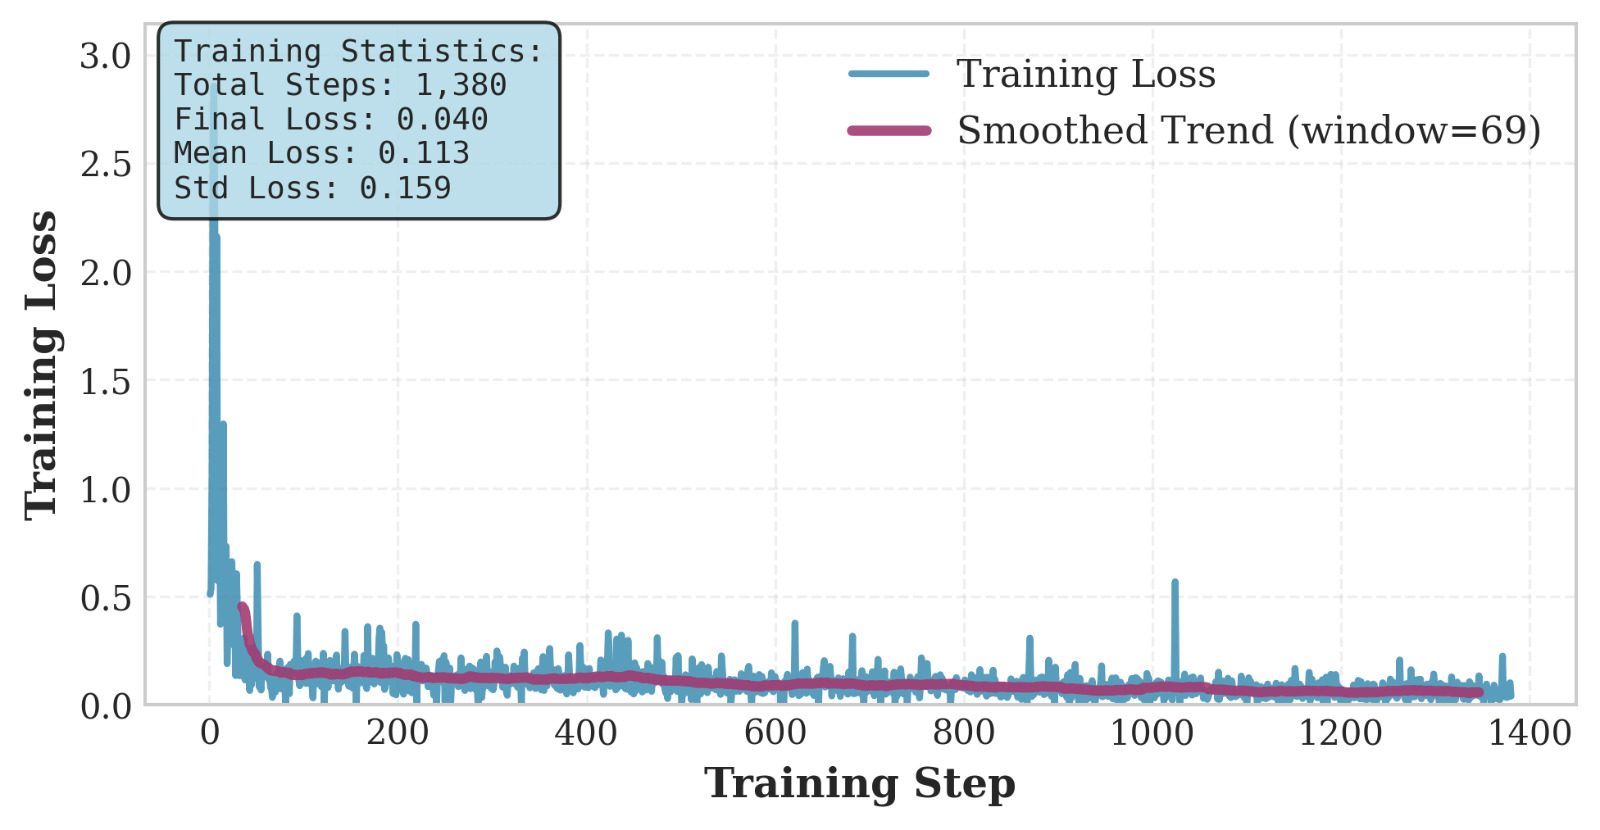
\includegraphics[width=\linewidth]{loss1.jpeg}
    \caption{The plot generated from the fine-tuning loss table provided by the OpenAI platform.}
    \label{fig:finetuning-loss}
\end{figure}

\subsubsection{Subtask 1A: Details results for reasoning model approach:} \label{appendix: 1AAgentic}

% Requires: \usepackage{colortbl}
\begin{table}[H]
    \centering
    \begin{tabular}{llr}
    \hline
 \textbf{Model Name} & \textbf{Reasoning Effort} & \textbf{Score} \\ \hline
    GPT-5 Nano & low & 0.82 \\ 
    O3 & high & 0.82 \\ 
    GPT-5 & low & 0.81 \\ 
    GPT-5 Nano & high & 0.81 \\ 
    GPT-5 Nano & medium & 0.81 \\ 
    O4 Mini & high & 0.81 \\ 
    GPT-5 & high & 0.79 \\ 
    O3 Mini & high & 0.79 \\
    GPT-5 & medium & 0.77 \\ 
    GPT-5 Mini & high & 0.76 \\ 
    GPT-5 & low & 0.70 \\ 
    GPT-5 Mini & medium & 0.65 \\ 
    GPT-5 Mini & high & 0.63 \\ \hline
    \end{tabular}
    \caption{Performance of the AI reasoning model with access to tools was evaluated under varying levels of reasoning effort, using models of different sizes}
    \label{tab:model_performance}
\end{table}
From Table \ref{tab:model_performance}, we note that smaller models and tiny models can outperform larger models for such specialized tasks.

\subsection{Subtask 2 evaluation on train and evaluation datasets}
For Subtask 2 see Table ~\ref{tab:subtask2_app}, we use the organizers’ code unmodified. Because train/dev lack hadith gold, our combined qrels capture Quran supervision only; hadith\_sample.qrels remains empty, hence MAP\_H@5 is 0 by construction. 
Evaluation results (merged train + dev Qrels): MAP@10=0.6199, MAP\_Q@5=0.5761, MAP\_H@5=0.0000 (expected given missing hadith gold).
\begin{table}[H]
\resizebox{\linewidth}{!}{
  \begin{tabular}{llll}
    \hline
    \textbf{\small{Approach}}           & \textbf{\small{MAP@10}} & \textbf{\small{MAP\_Q@5}}  & \textbf{\small{MAP\_H@5}}   		\\
    \hline
    RAG-based(dev+train datasets)        &  0.6199       &  0.5761   &         0.0000                      \\
    RAG-based(benchmark)   &  0.2807       &  0.3257   &          0.2386    
 \\

 \hline
  \end{tabular}
  }
  \caption{\label{tab:subtask2_app}
    Subtask 2 evaluation results. 
  }
\end{table}


\end{document}
